\documentclass[11pt]{article}
\usepackage[utf8]{inputenc}
\usepackage[english]{babel}
\usepackage{amsmath}
\usepackage{graphicx}
\usepackage{float}
\usepackage{lipsum}
\usepackage{multicol}
\usepackage{xcolor}
\usepackage{tabularx}
\usepackage{tikz}
\usepackage{booktabs}
\usepackage{float}
\usepackage{hyperref}
\usepackage{caption}
\usepackage{enumitem}

\newcolumntype{Y}{>{\centering\arraybackslash}X}
\usepackage[left=1.90cm, right=1.90cm, top=1.00cm, bottom=1.75cm]{geometry}

\title{AN2DL Reports Template}

\begin{document}
    \begin{figure}[H]
    \begin{minipage}[c]{0.5\textwidth}
        \vspace{1cm}% Takes up the left half of the page
        \flushleft % Aligns the image to the far left
        
\includegraphics[scale=0.5]{polimi.png}
    \end{minipage}
    \begin{minipage}[c]{0.5\textwidth}
            \vspace{1cm}
        \flushright 
        
\includegraphics[scale=0.3]{airlab.jpeg}
    \end{minipage}
    \end{figure}
    
    \begin{center}
        % Select between First and Second
        \vspace{-3cm}
        {\Large \textbf{AN2DL - First Challenge Report}}\\
        \vspace{2mm}
        % Change with your Team Name
        {\Large \textbf{ReLUctant}}\\
        \vspace{2mm}
        % Team Members Information
        {\large Alessandro Del Fatti,}
        {\large Matteo Garzone,}
        {\large Francesco Genovese} \\ 
        \vspace{2mm}
        % Codabench Nicknames
        {Kaggle: alessandrodelfatti,}
        {matteogarzone,}
        {frncscgnvs} \\
        \vspace{2mm}
        % Matriculation Numbers
        {270240,}
        {279709,}
        {307916} \\
        \vspace{2mm}
        \today
    \end{center}    
    \setlength{\columnsep}{1cm}
    \begin{multicols}{2}
    
        \section{Introduction}
        % In this section, you should present your project's context and objectives. You might want to:
        % \begin{itemize}
        %     \item Define the problem (\textit{you may use italics to highlight definitions})
        %     \item State your goals (\textbf{emphasise key points with bold})
        %     \item Outline your approach
        % \end{itemize}
        
        % \noindent For instance, you might write: ``This project focuses on \textit{image classification} using \textbf{deep learning} techniques."
        
        This report presents our approach to the AN2DL course first challenge, tackling a supervised deep learning task on the \textit{Pirates Pain} dataset. 
        
        The presented problem is a a multiclass time series classification with the objective to predict pain levels experienced by pirates based on the biomechanical sensor data provided. 
       
        %\begin{figure}[H] % 1. Use a 'figure' environment
        %    \centering % Good practice to center it
        %    \begin{tikzpicture}
                
                % 1. Define the clipping path first
        %        \clip [rounded corners=1cm] (0,0) rectangle (0.9\linewidth, 3.8cm); 
                
                % 2. Place the node at the center of the clip path
                %    (0.9\linewidth / 2 = 0.45\linewidth, 4.5cm / 2 = 2.25cm)
        %        \node [inner sep=0pt] at (0.45\linewidth, 1.9cm) {
                    
                    % 3. Set image width to match the clip width
        %            
\includegraphics[width=0.9\linewidth]{header.png}
        %        };
        
        %    \end{tikzpicture}
            
            % 4. Place the caption INSIDE the figure, but OUTSIDE tikzpicture
        %    \caption{Arrr my legeth}
        %    \label{fig:my-header} % Optional: add a label for cross-referencing
        % \end{figure}
        
        The task involves classifying pain into three categories: \textbf{No Pain} (class 0), \textbf{Low Pain} (class 1), and \textbf{High Pain} (class 2). 

        
        The challenge presents significant difficulties due to severe class imbalance (77\% No Pain, 14\% Low Pain, 9\% High Pain), high-dimensional temporal data, and the need to capture temporal dependencies in the data.
        \vspace{-3mm}
        \section{Data profiling and feature engineering}
        Before starting the training process of the model, we decided to perform a first step of data profiling. In particular, we took advantage of the {\texttt{YDataProfiling} Python library}\footnote{https://docs.profiling.ydata.ai/}. Using this tool, we noticed that in the dataset:
        \begin{itemize}
            \setlength{\itemsep}{1pt}
            \setlength{\parskip}{0pt}
            \setlength{\parsep}{0pt}
            \item Feature \texttt{joint\_30} is constant. We decided to remove it, as it provides no information.
            \item Features \texttt{n\_legs}, \texttt{n\_hands}, and \texttt{n\_eyes} are shared among pirates; that is, if a pirate only has 1 leg, they also have 1 hand and a patch over one eye. We decided to merge them into a unique feature called \texttt{has\_prosthesis}.
            \item Many features in the set of \texttt{joint\_xx} are found to be \textbf{highly correlated}, as reported by the heatmap in figure \ref{heatmap-correlation}. To handle this, we decided to compute the average of the columns that showed a correlation higher than a certain threshold (we decided to set it to $0.8$).
        \end{itemize}
        %\vspace{-0.5cm}
        \begin{center}
            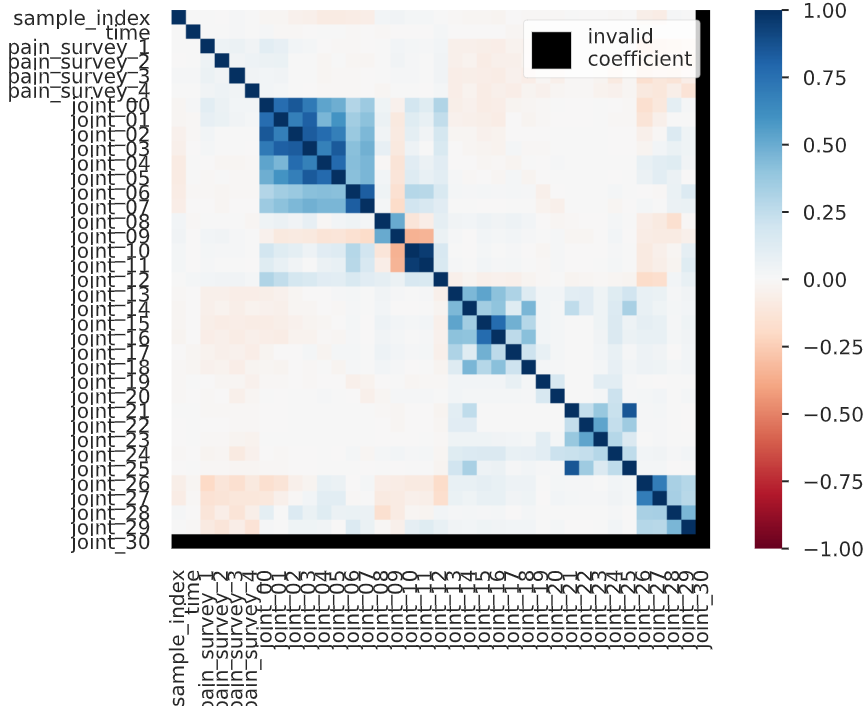
\includegraphics[scale=0.25]{heatmap-correlation.png}
            \captionof{figure}{Heatmap of the correlations between features}
            \label{heatmap-correlation}
        \end{center}
        In addition to the profiling analysis, we computed the autocorrelation function (ACF) for the numerical features. The average \textbf{first negative lag} was $29.93$, the first lag with $|ACF| < 0.1$ was $4.60$, and the \textbf{average maximum peak lag} was $ 1.26$. The ACF provided valuable insights into the temporal dependencies of our data and helped improve model performance. However, since the ACF was computed following the logbook’s suggestion after an initial, time-consuming grid search for selecting the window size and stride hyperparameters, the window size values from the grid search reported in \ref{grid-search} do not fully align with the ACF insights. 
        
        At last, during training, we used the window size hyperparameter values suggested by the ACF, which proved to be around $10$
        % \section{Problem Analysis}
        % Here you can discuss your initial analysis of the problem. Consider including:
        % \begin{enumerate}
        %     \item Dataset characteristics
        %     \item Main challenges
        %     \item Initial assumptions
        % \end{enumerate}

        % \noindent If you need to reference papers, use the citation command: Recent work~\cite{lecun2015deep} suggests..."

        \section{Method}
        % This section should detail your approach. You can use equations to explain your methodology. For example, a simple model representation:
        % \begin{equation}
        %     \label{eq:model}
        %     f(x) = \text{softmax}(Wx + b)
        % \end{equation}

        % \noindent Or a more complex loss function:
        % \begin{equation}
        %     \label{eq:loss}
        %     \mathcal{L} = -\frac{1}{N}\sum_{i=1}^{N} y_i\log(\hat{y}_i)
        % \end{equation}

        % \noindent Reference these equations in your text, like:``As shown in equation~\ref{eq:model}..."

        %%\color{red}\textbf{TO CHECK! }\color{black}
        \subsection{Preprocessing Pipeline}
        Our preprocessing pipeline consists of several critical steps:
            
        \textbf{1. Normalization:} We applied minmax normalization to all features to avoid gradient explosion.
        $$x_{\text{normalized}} = \frac{x - \min(x)}{\max(x) - \min(x)}$$
        %%QUESTION: did we use this or standard normalization
        %%TODO insert formulas
        
        \textbf{2. Temporal Encoding:}
        Added cyclical time-position encoding features to capture sequence progression. With $P$ set to obtain days and weekdays.
        $$x_{\sin} = \sin\left(\frac{2\pi x}{P}\right) , \ \ x_{\cos} = \cos\left(\frac{2\pi x}{P}\right)$$

        %%TODO insert forumlas
        
        \textbf{3. Sequence Windowing:}
        Applied sliding windows with a \texttt{size=10} and \texttt{stride=5} to create shorter sequences:
        \begin{equation}
            S_i = [x_{i \cdot stride}, ..., x_{i \cdot stride + window-1}]
        \end{equation}
        
        This increased the number of samples for the training and validation steps.

         \subsection{Data Augmentation}
        To address class imbalance, we applied targeted oversampling of minority classes. We tried two approaches:
        \begin{itemize}
            \setlength{\itemsep}{1pt}
            \setlength{\parskip}{0pt}
            \setlength{\parsep}{0pt}
            \item Computation of inverse-proportional class weights for loss function weighting
            \item Oversampling of the less populated classes
        \end{itemize}
        
        \subsection{Training Strategy}
        \subsubsection{Loss Function:}
        \textit{Categorical cross-entropy} with class weights computed for minority class oversampling.
        We also experimented with:
        \begin{itemize}[noitemsep,topsep=0pt]
            \setlength{\itemsep}{1pt}
            \setlength{\parskip}{0pt}
            \setlength{\parsep}{0pt}
            \item  \textit{Label Smoothing loss:} a custom made categorical cross-entropy extension that also maps class labels to properly-distanced floats rather than equally-distanced integers.
            \item \textit{Focal loss:} a categorical cross-entropy extension designed to address class imbalance in classification tasks by giving higher weights to hard-to-classify data samples while down-weighting samples classified with higher confidence. 
        \end{itemize}

        \subsubsection{Regularization Techniques:}
        We performed a grid search in four steps, obtaining  best performance with the configurations in table \ref{grid-search}. For complete reference, consult the training logs in the notebooks. We noticed that, to achieve better performance in terms of F1-score, \textbf{a small window size} (as discussed before) \textbf{and low values for the regularization terms $\ell_1$ and $\ell_2$ are preferable}. So, starting from those values, we tried to further reduce them, obtaining better results:
        %%TODO Sistemare formatting
        \begin{itemize}[noitemsep,topsep=0pt]
            \setlength{\itemsep}{1pt}
            \setlength{\parskip}{0pt}
            \setlength{\parsep}{0pt}
            \item $\ell_1$ regularization: best if turned off.
            \item $\ell_2$ regularization: $1e-5$
            \item Dropout: 0.2 @ CNN-1d, 0.4 @ LSTM \color{red}check, is it not 0.3?\color{black}
        \end{itemize}
        We also experimented with:
        \begin{itemize}[noitemsep,topsep=0pt]
            \setlength{\itemsep}{1pt}
            \setlength{\parskip}{0pt}
            \setlength{\parsep}{0pt}
            \item Label smoothing: $\alpha = 0.1$
            \item Gradient clipping and normalization: $max_{|\nabla L|}=1.0$
        \end{itemize}


        \subsubsection{Optimization:}
        %%TODO Sistemare formatting
        \begin{itemize}[noitemsep,topsep=0pt]
            \setlength{\itemsep}{1pt}
            \setlength{\parskip}{0pt}
            \setlength{\parsep}{0pt}
            \item Optimizer: AdamW
            \item Learning rate: $3 \times 10^{-4}$
            \item Batch size: 64
            \item Early stopping: \texttt{patience=50} epochs on validation F1
            \item LR scheduler: \texttt{ReduceLROnPlateau(factor=0.5, patience=40)}
        \end{itemize}
        
        \section{Experiments}
        % For your experiments, you might want to present your results in tables. Here's an example of a wide table comparing different models:
        As a first approach, we tried using baseline models: RNN, LSTM, GRU and their relative bidirectional versions. By evaluating them, we noticed that the \textbf{bidirectional LSTM} performs better consistently, across different configurations of hyperparameters.

        \begin{table}[H]
            \centering
            \resizebox{3.5cm}{!}{%
            \begin{tabular}{c | c}
                Model & Val F1\\
                \hline
                RNN & 0.6294\\
                Bi-RNN & 0.8539 \\
                LSTM & 0.6294 \\
                Bi-LSTM & \textbf{0.9472} \\
                GRU & 0.6294 \\
                Bi-GRU & 0.8651 \\
            \end{tabular}
            }
        \end{table}
        

        After choosing a model, we used grid search to find a good set of hyperparameters for the network.

        Since our model was lacking accuracy on the less populated class (\textbf{High pain}), we tried to address the problem by implementing  sample augmentation and using loss functions that scale up errors in minority classes.

        Lastly, adding a 1D Convolutional layer and an Attention layer to the network, resulted in improved performance.
        
        We experimented with a \textbf{hierarchical classification} approach: we used a binary classifier to discriminate \textbf{No Pain} from \textbf{Pain} labeled samples and a second binary classifier to distinguish the levels of pain \textbf{High} and \textbf{Low} of samples classified as painful. This approach proved to be overfitting for the hyperparameter set we used, but sure is a promising path to be explored for such a task.
        
        
        % \begin{table*}[t]
        %     \centering
        %     \setlength{\tabcolsep}{5pt}
        %     \caption{An example of wide table. Best results are highlighted in \textbf{bold}.}
        %     \begin{tabularx}{\textwidth}{lYYYc}
        %         \toprule
        %         Model & Accuracy & Precision & Recall & ROC AUC\\
        %         \midrule
        %         VGG18         &  72.20 $\pm$ 3.06    &   94.95 $\pm$ 0.52     &   86.95 $\pm$ 0.55    &   80.16 $\pm$ 0.81\\
        %         Custom Model        &  27.71 $\pm$ 3.19    &   75.70 $\pm$ 1.07     &   55.75 $\pm$ 2.16    &   36.60 $\pm$ 1.26\\
        %         ResNet18    &  \textbf{89.24 $\pm$ 2.38}    &   \textbf{95.54 $\pm$ 0.49}     &   \textbf{93.43 $\pm$ 1.30}    &   \textbf{91.68 $\pm$ 0.71}\\
        %         \bottomrule
        %     \end{tabularx}
        %     \label{tab:Performance}
        % \end{table*}

        % \noindent For more specific measurements, you might use a narrower table:
    
        % \begin{table}[H]
        %     \centering
        %     \setlength{\tabcolsep}{3pt}
        %     \caption{An example of table. Best results may be highlighted in \textbf{bold}.}
        %     \begin{tabularx}{\linewidth}{lY}
        %         \toprule
        %         Time [$\mu$s] & Distance [mm]\\
        %         \midrule
        %         22$\pm$4 & 8$\pm$1\\
        %         17$\pm$3 & 7$\pm$1\\
        %         15$\pm$3 & 6$\pm$1\\
        %         13$\pm$2 & 5$\pm$1\\
        %         10$\pm$2 & 4$\pm$1\\
        %         8$\pm$2 & 3$\pm$1\\
        %         5$\pm$1 & 2$\pm$1\\
        %         37$\pm$1 & 1$\pm$1\\
        %         \bottomrule
        %     \end{tabularx}
        %     \label{tb:Measurements}
        % \end{table}

        % \noindent You can also include figures to visualise your results:
        % \begin{figure}[H]
        %     \centering
        %     
\includegraphics[width=0.75\linewidth]{random.jpeg}
        %     \caption{Example figure showing [describe what the figure shows]}
        %     \label{fig:results}
        % \end{figure}

        % \noindent Reference figures using like:``As shown in Figure~\ref{fig:results}..."

        \section{Results}
        % Present your main findings here. You might want to:
        % \begin{itemize}
        %     \item Compare your results with baselines
        %     \item Highlight key achievements using \textbf{bold text}
        %     \item Explain any unexpected outcomes
        % \end{itemize}
        We experimented with different model configurations, gradually adding modules and features.

        As table \ref{tab:model_comparison} suggests, a bidirectional LSTM based classifier with a convolutional and an attention layer, which takes into account temporal features as well, trained with gradient clipping, LR scheduling, and minority classes oversampling, is the best performing.
        
        

        \section{Discussion}
        % In this section, analyse your results critically. Consider:
        % \begin{itemize}
        %     \item Strengths and weaknesses
        %     \item Limitations and assumptions
        % \end{itemize}

        \subsection{Strengths of Our Approach}
        \begin{enumerate}[noitemsep,topsep=0pt]
            \setlength{\itemsep}{1pt}
            \setlength{\parskip}{0pt}
            \setlength{\parsep}{0pt}
            \item \textbf{Code modularity: } Having our project set up in modules that load configuration files for training, using the notebook only as a training pipeline helped us to add functionality, debug, and compare approaches easily. 
        \item \textbf{Robustness:} Consistent performance despite severe class imbalance.
            \item \textbf{Proper Model Selection:} Chose a simpler model over a higher validation score.
        \end{enumerate}
        \subsection{Limitations and Lessons Learned}
        \begin{enumerate}[noitemsep,topsep=0pt]
            \setlength{\itemsep}{1pt}
            \setlength{\parskip}{0pt}
            \setlength{\parsep}{0pt}
            \item \textbf{Augmentation Risk:} Aggressive augmentation can create unrealistic patterns that do not generalize.
            \item \textbf{Hierarchical Overfitting:} High validation scores do not guarantee test performance.
            \item \textbf{Data analysis:} the usefulness of ACF computation in time series analysis is evident. In retrospect, conducting a thorough dataset profiling before performing the grid search would likely have been more beneficial.
        \end{enumerate}
        \section{Conclusions}
        % Summarise your work and discuss potential future directions. This is where you can:
        % \begin{itemize}
        %     \item Restate main contributions
        %     \item Suggest improvements
        %     \item Propose future work
        % \end{itemize}
        %\bibliography{references}
        This work addressed the task through a comprehensive approach, combining data profiling with feature and NN architecture engineering. Our final model achieved a test weighted F1-score of 0.9616 on the provided open test set, demonstrating strong generalization despite severe class imbalance.

        Key contributions include systematic feature engineering guided by profiling, correlation analysis, and ACF computation; effective handling of class imbalance through targeted oversampling and weighted loss functions; a modular code architecture that facilitated rapid experimentation and hyperparameter optimization.
        
        Future work could explore advanced augmentation techniques specifically designed for biomechanical time series, ensemble methods combining multiple architectures, and further refinement of the hierarchical classification approach to reduce overfitting while maintaining its validation performance advantage.
        
    
        \bibliographystyle{abbrv}
    \end{multicols}
    
    
        
       \begin{table*}[ht]
            \centering
            \resizebox{14cm}{!}{%
            \begin{tabular}{c|c|c||c|c|c}
                \textbf{Window Size} & \textbf{Stride} & \textbf{F1 Score} &
                \textbf{Batch Size} & \textbf{Learning rate} & \textbf{F1 Score} \\
                \hline
                50  & 25 & 0.9181 $\pm$ 0.0327 &
    %            32  & 1e-4 & 0.9196 $\pm$ 0.0335 \\
                
    %            50  & 50 & 0.8945 $\pm$ 0.0399 &
    %            32  & 3e-4 & 0.9238 $\pm$ 0.0392 \\
    %            
    %            100 & 25 & 0.9087 $\pm$ 0.0406 &
    %            32  & 1e-3 & 0.9172 $\pm$ 0.0332 \\
                
    %            100 & 50 & 0.9028 $\pm$ 0.0380 &
    %            64  & 1e-4 & 0.9139 $\pm$ 0.0348 \\
                
    %            200 & 25 & 0.8748 $\pm$ 0.0381 &
                64  & 3e-4 & 0.9250 $\pm$ 0.0329 \\
                
    %            200 & 50 & 0.8713 $\pm$ 0.0461 &
    %            64  & 1e-3 & 0.9212 $\pm$ 0.0437 \\
            \end{tabular}
            }
    %        \caption{Grid search: step 1 (left) and 2 (right)}
    %        \label{grid-search-1}
            
    %\end{table*}

         \vspace{0.5cm}

    %    \begin{table*}[ht]
    %        \centering
            \resizebox{14cm}{!}{%
            \begin{tabular}{c|c|c||c|c|c|c}
                \textbf{Hid. layers} & \textbf{Hid. size} & \textbf{F1 Score} &
                \textbf{$\ell_1$} & \textbf{$\ell_2$} & \textbf{Dropout} & \textbf{F1 Score} \\
                \hline
    %            1 & 64 & 0.9120 $\pm$ 0.0349 &
    %            1e-4  & 1e-4 & 0.2 & 0.9161 $\pm$ 0.0349 \\
                
    %            1  & 128 & 0.9170 $\pm$ 0.0310 &
                1 & 256 & 0.9314 $\pm$ 0.0361 &
                1e-4  & 1e-4 & 0.4 & 0.9168 $\pm$ 0.0371 \\
                
    %            \textbf{1} & \textbf{256} & \textbf{0.9314 $\pm$ 0.0361} &
    %            1e-4  & 1e-3 & 0.2 & 0.9023 $\pm$ 0.0152 \\
                
    %            2 & 64 & 0.9198 $\pm$ 0.0272 &
    %            1e-4  & 1e-3 & 0.4 & 0.9095 $\pm$ 0.0321 \\
                
    %            2 & 128 &0.9218 $\pm$ 0.0301 &
    %            1e-3  & 1e-4 & 0.2 & 0.8000 $\pm$ 0.0065 \\
                
    %            2 & 256 & 0.9211 $\pm$ 0.0275 &
    %            1e-3  & 1e-4 & 0.4 & 0.8278 $\pm$ 0.0372 \\

     %           3 & 64 & 0.9277 $\pm$ 0.0286 &
     %           1e-3 & 1e-3 & 0.2 & 0.8054 $\pm$ 0.0223 \\
                
     %           3  & 128 & 0.9232 $\pm$ 0.0252 &
     %           1e-3 & 1e-3 & 0.4 & 0.8182 $\pm$ 0.0217 \\
                
     %           3 & 256 & 0.9229 $\pm$ 0.0269 &
     %           & & & \\
            \end{tabular}
            }
            \caption{Grid search: best results obtained using the grid search in four steps}
            \label{grid-search}
        \end{table*}


        \begin{table*}[h] % <-- CHANGED [Ht] to [t!]
            \centering      
            \resizebox{14cm}{!}{
            \begin{tabular}{l|c|c|c|l}
                \textbf{Model} & \textbf{Val F1} & \textbf{Test F1} & \textbf{Params} & \textbf{Notes}\\ \hline
                
                Baseline Bi-LSTM (1hl, 256h) & 0.9168 & 0.9051 & 392K & Grid search hyperparameters \\
                Bi-LSTM + LRScheduling + L2 reg & 0.9232 & 0.9163 & 392K & Better regularization and convergence\\
                Bi-LSTM + CNN1d & 0.9288 & 0.9142 & 855K & Added CNN 1d layer\\
                
                Bi-LSTM + Temp + CNN1d & 0.9305 & 0.9208 & 855K & Temporal features added \\
                \textbf{Bi-LSTM + Temp + CNN1d + Attention} & \textbf{0.9312} & \textbf{0.9616} & \textbf{878K} & Added an attention layer \\
                Hierarchical 2-Step classifier & 0.9925 & 0.9293 & 856K & Overfitting\\
            \end{tabular}
            }
            \caption{Performance comparison of different model configurations. Best results in bold}
            \label{tab:model_comparison}
        \end{table*}
        
\end{document}